
\begin{figure*}
	\centering
	\begin{subfigure}[t]{0.32\textwidth}
		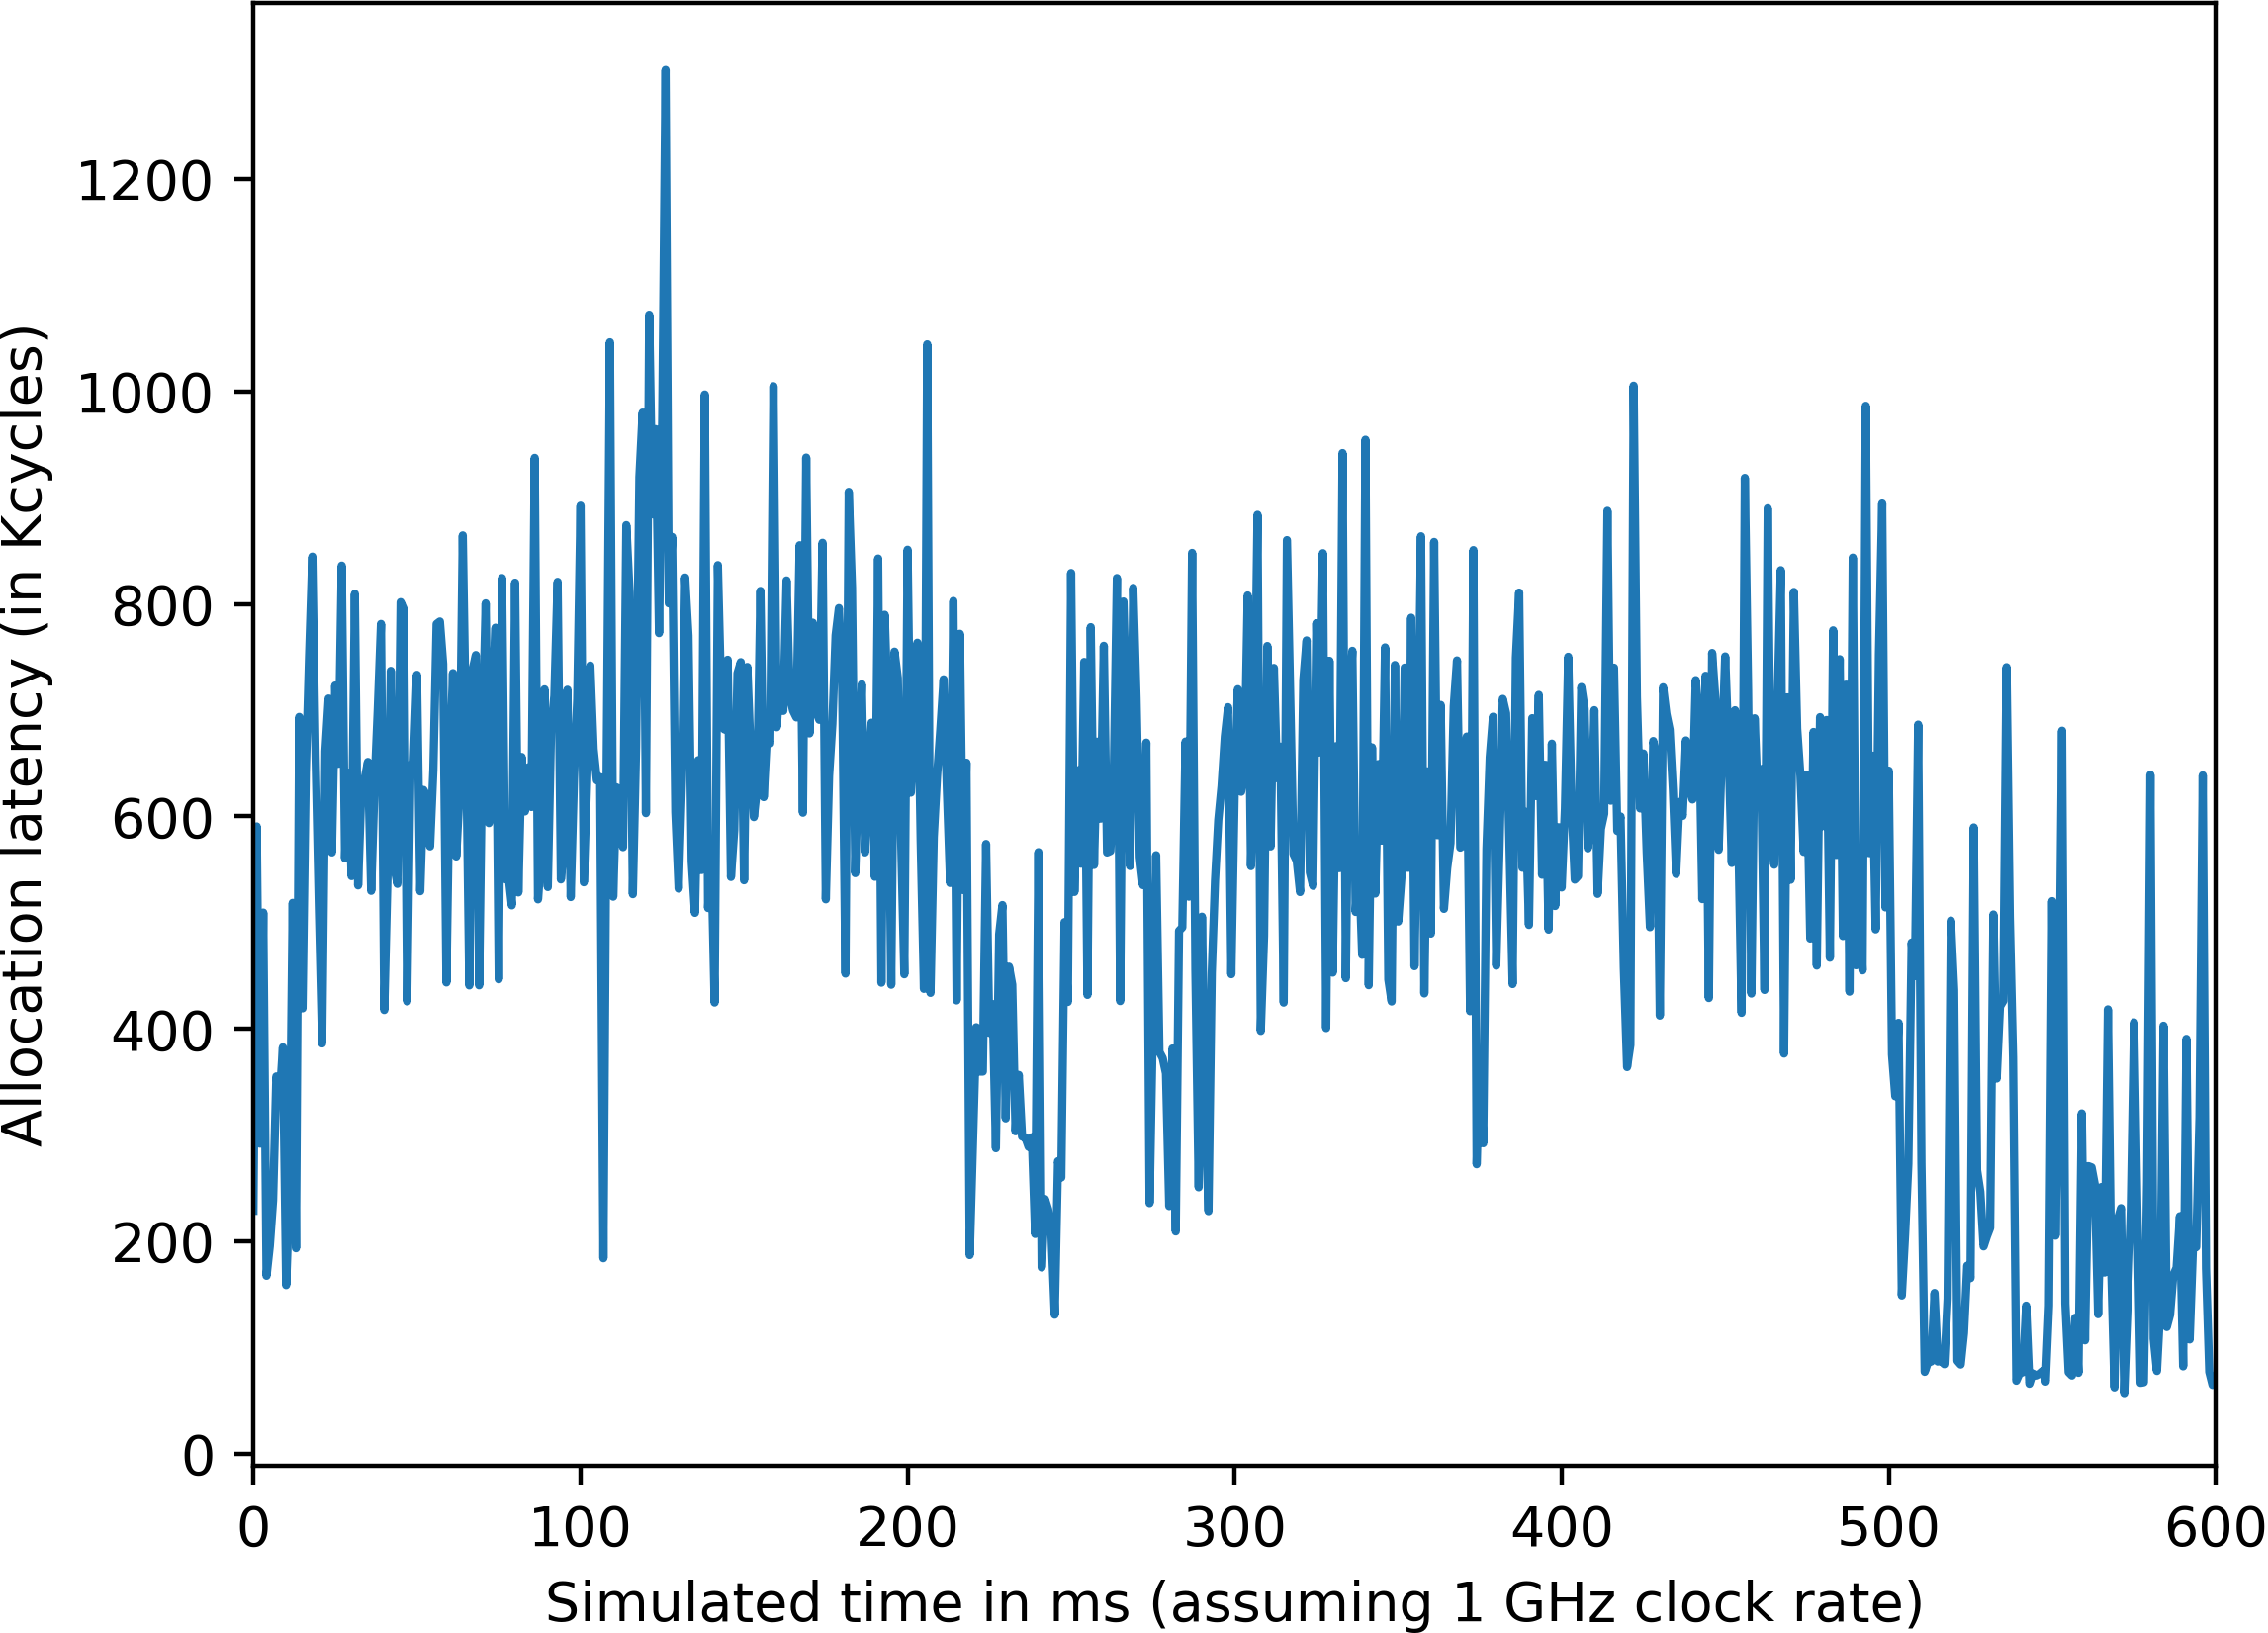
\includegraphics[width=\textwidth]{results/java-alloc-macro.png}
		\caption{The first 600ms of execution sampled at 1 KHz}
	\end{subfigure}
	\begin{subfigure}[t]{0.32\textwidth}
		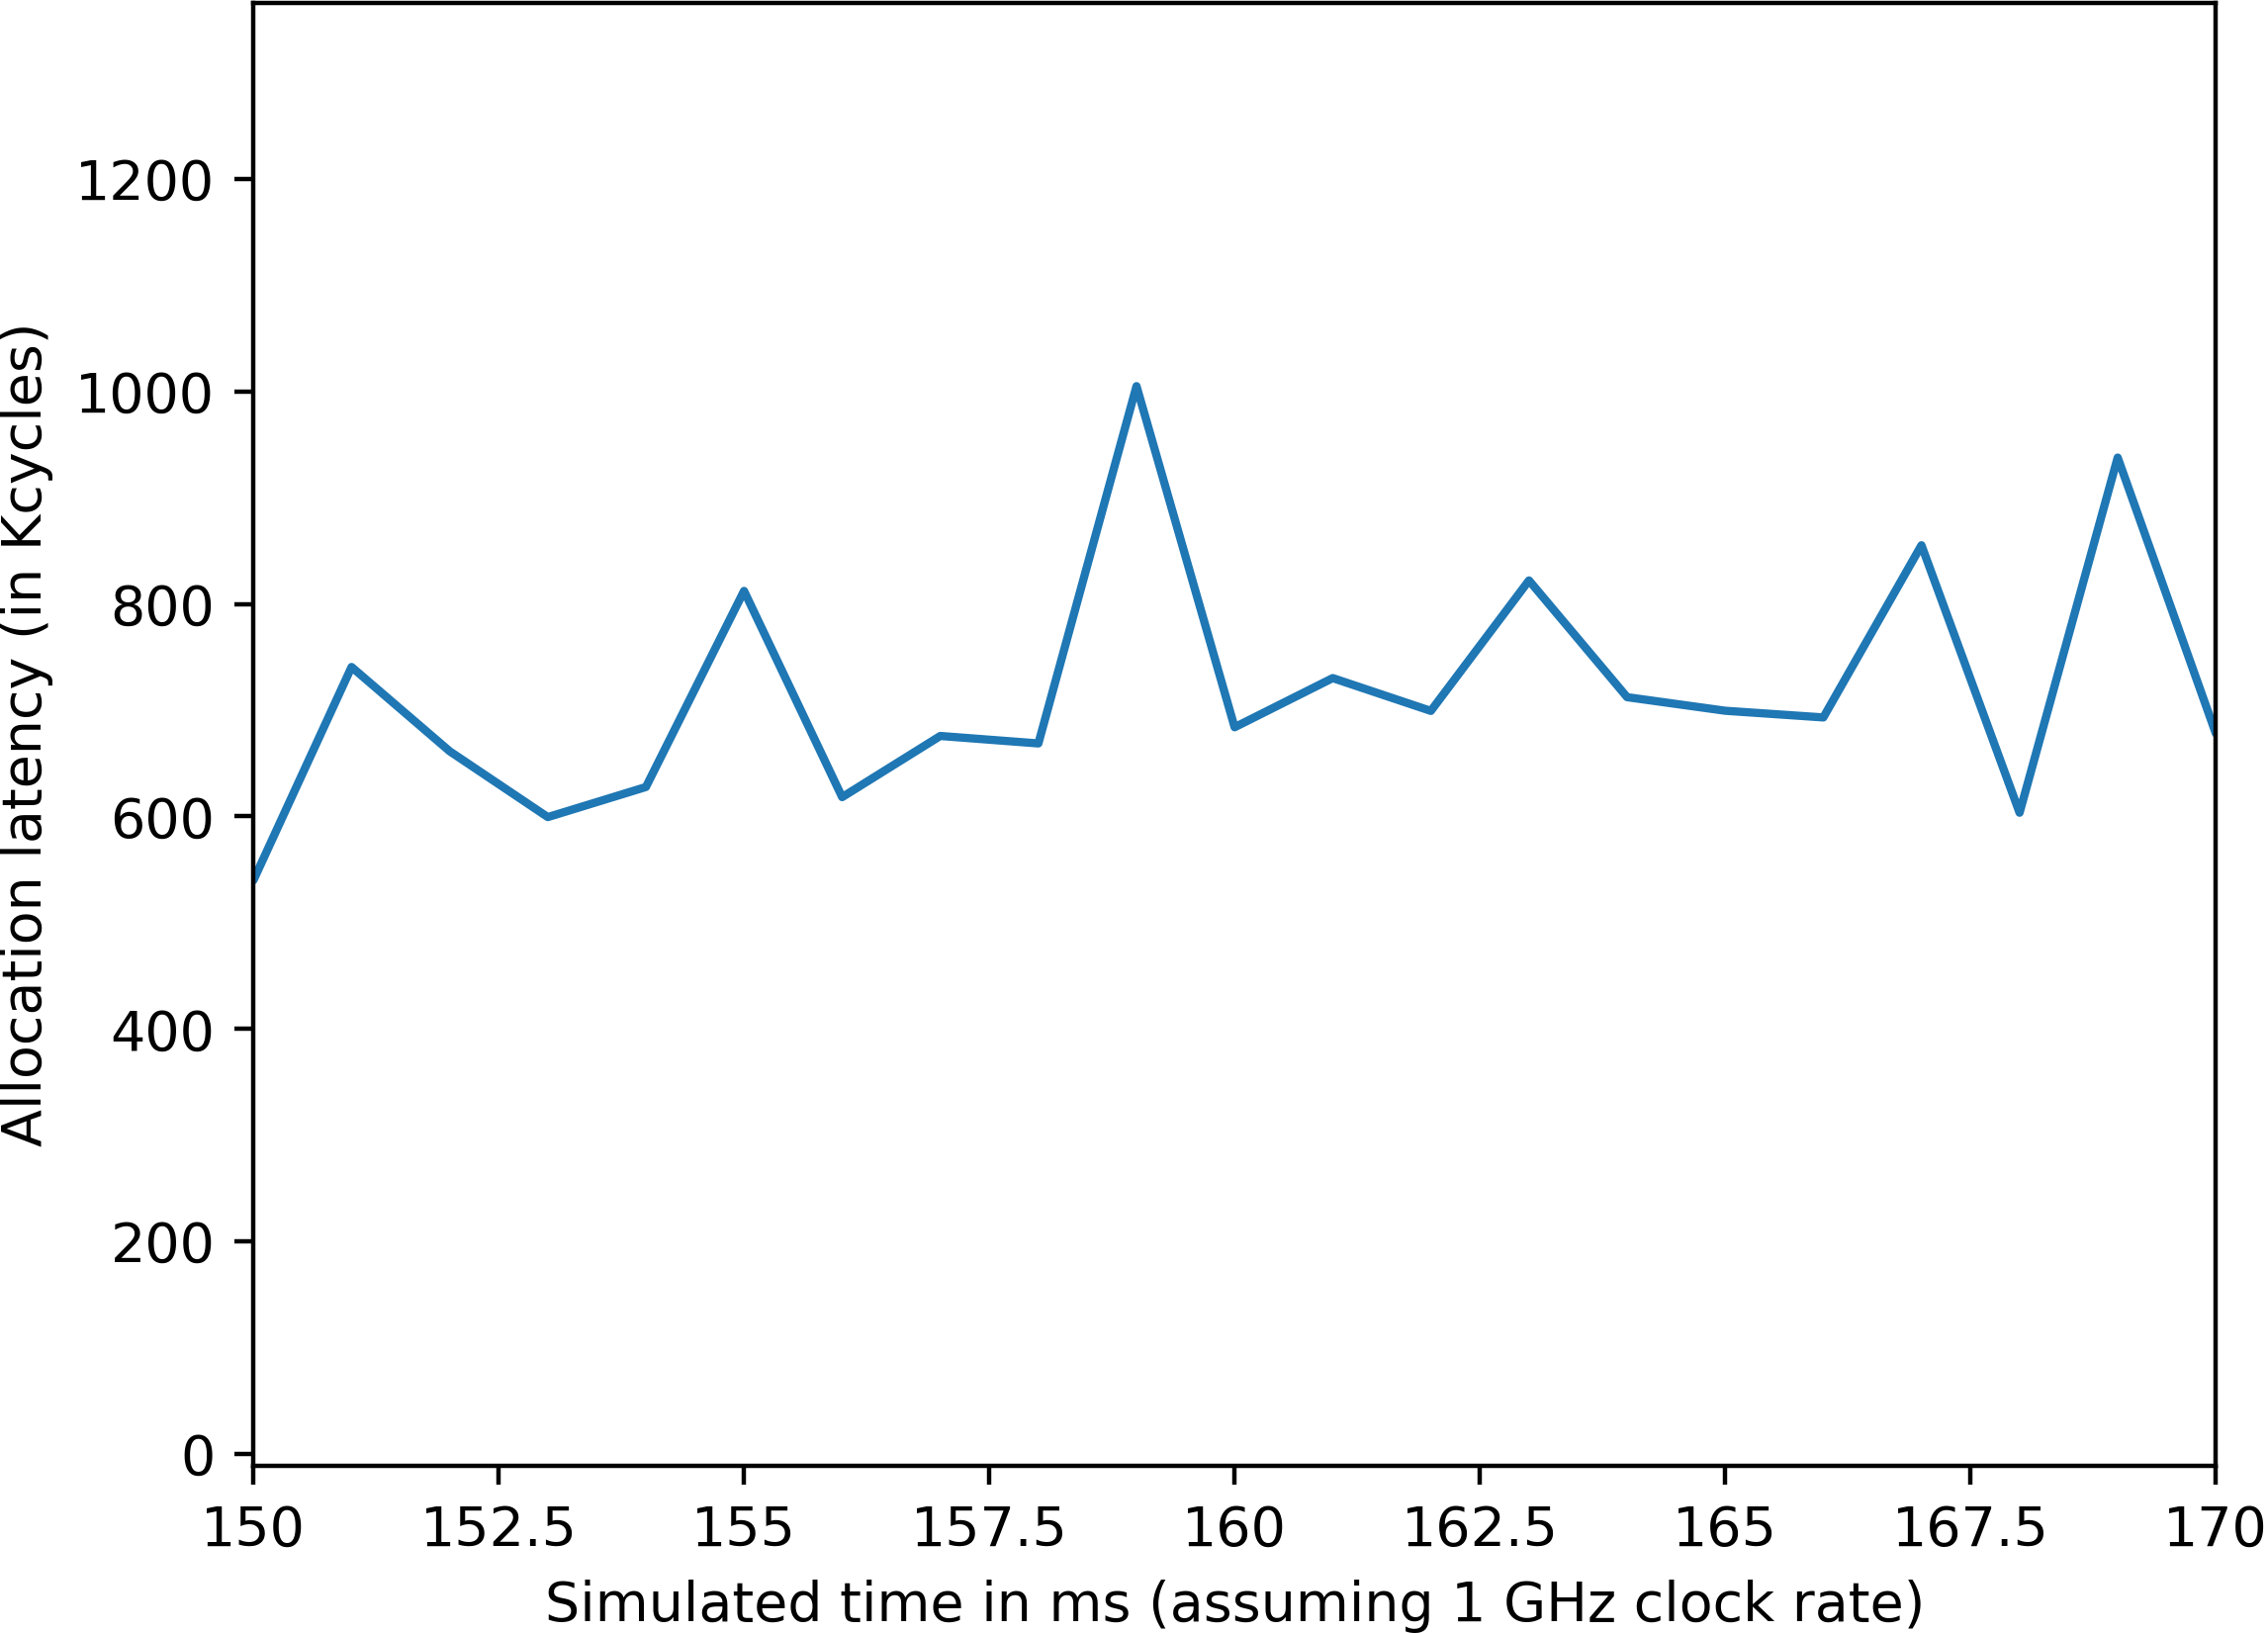
\includegraphics[width=\textwidth]{results/java-alloc-1khz.png}
		\caption{20ms slice sampled at 1 KHz}
	\end{subfigure}
	\begin{subfigure}[t]{0.32\textwidth}
		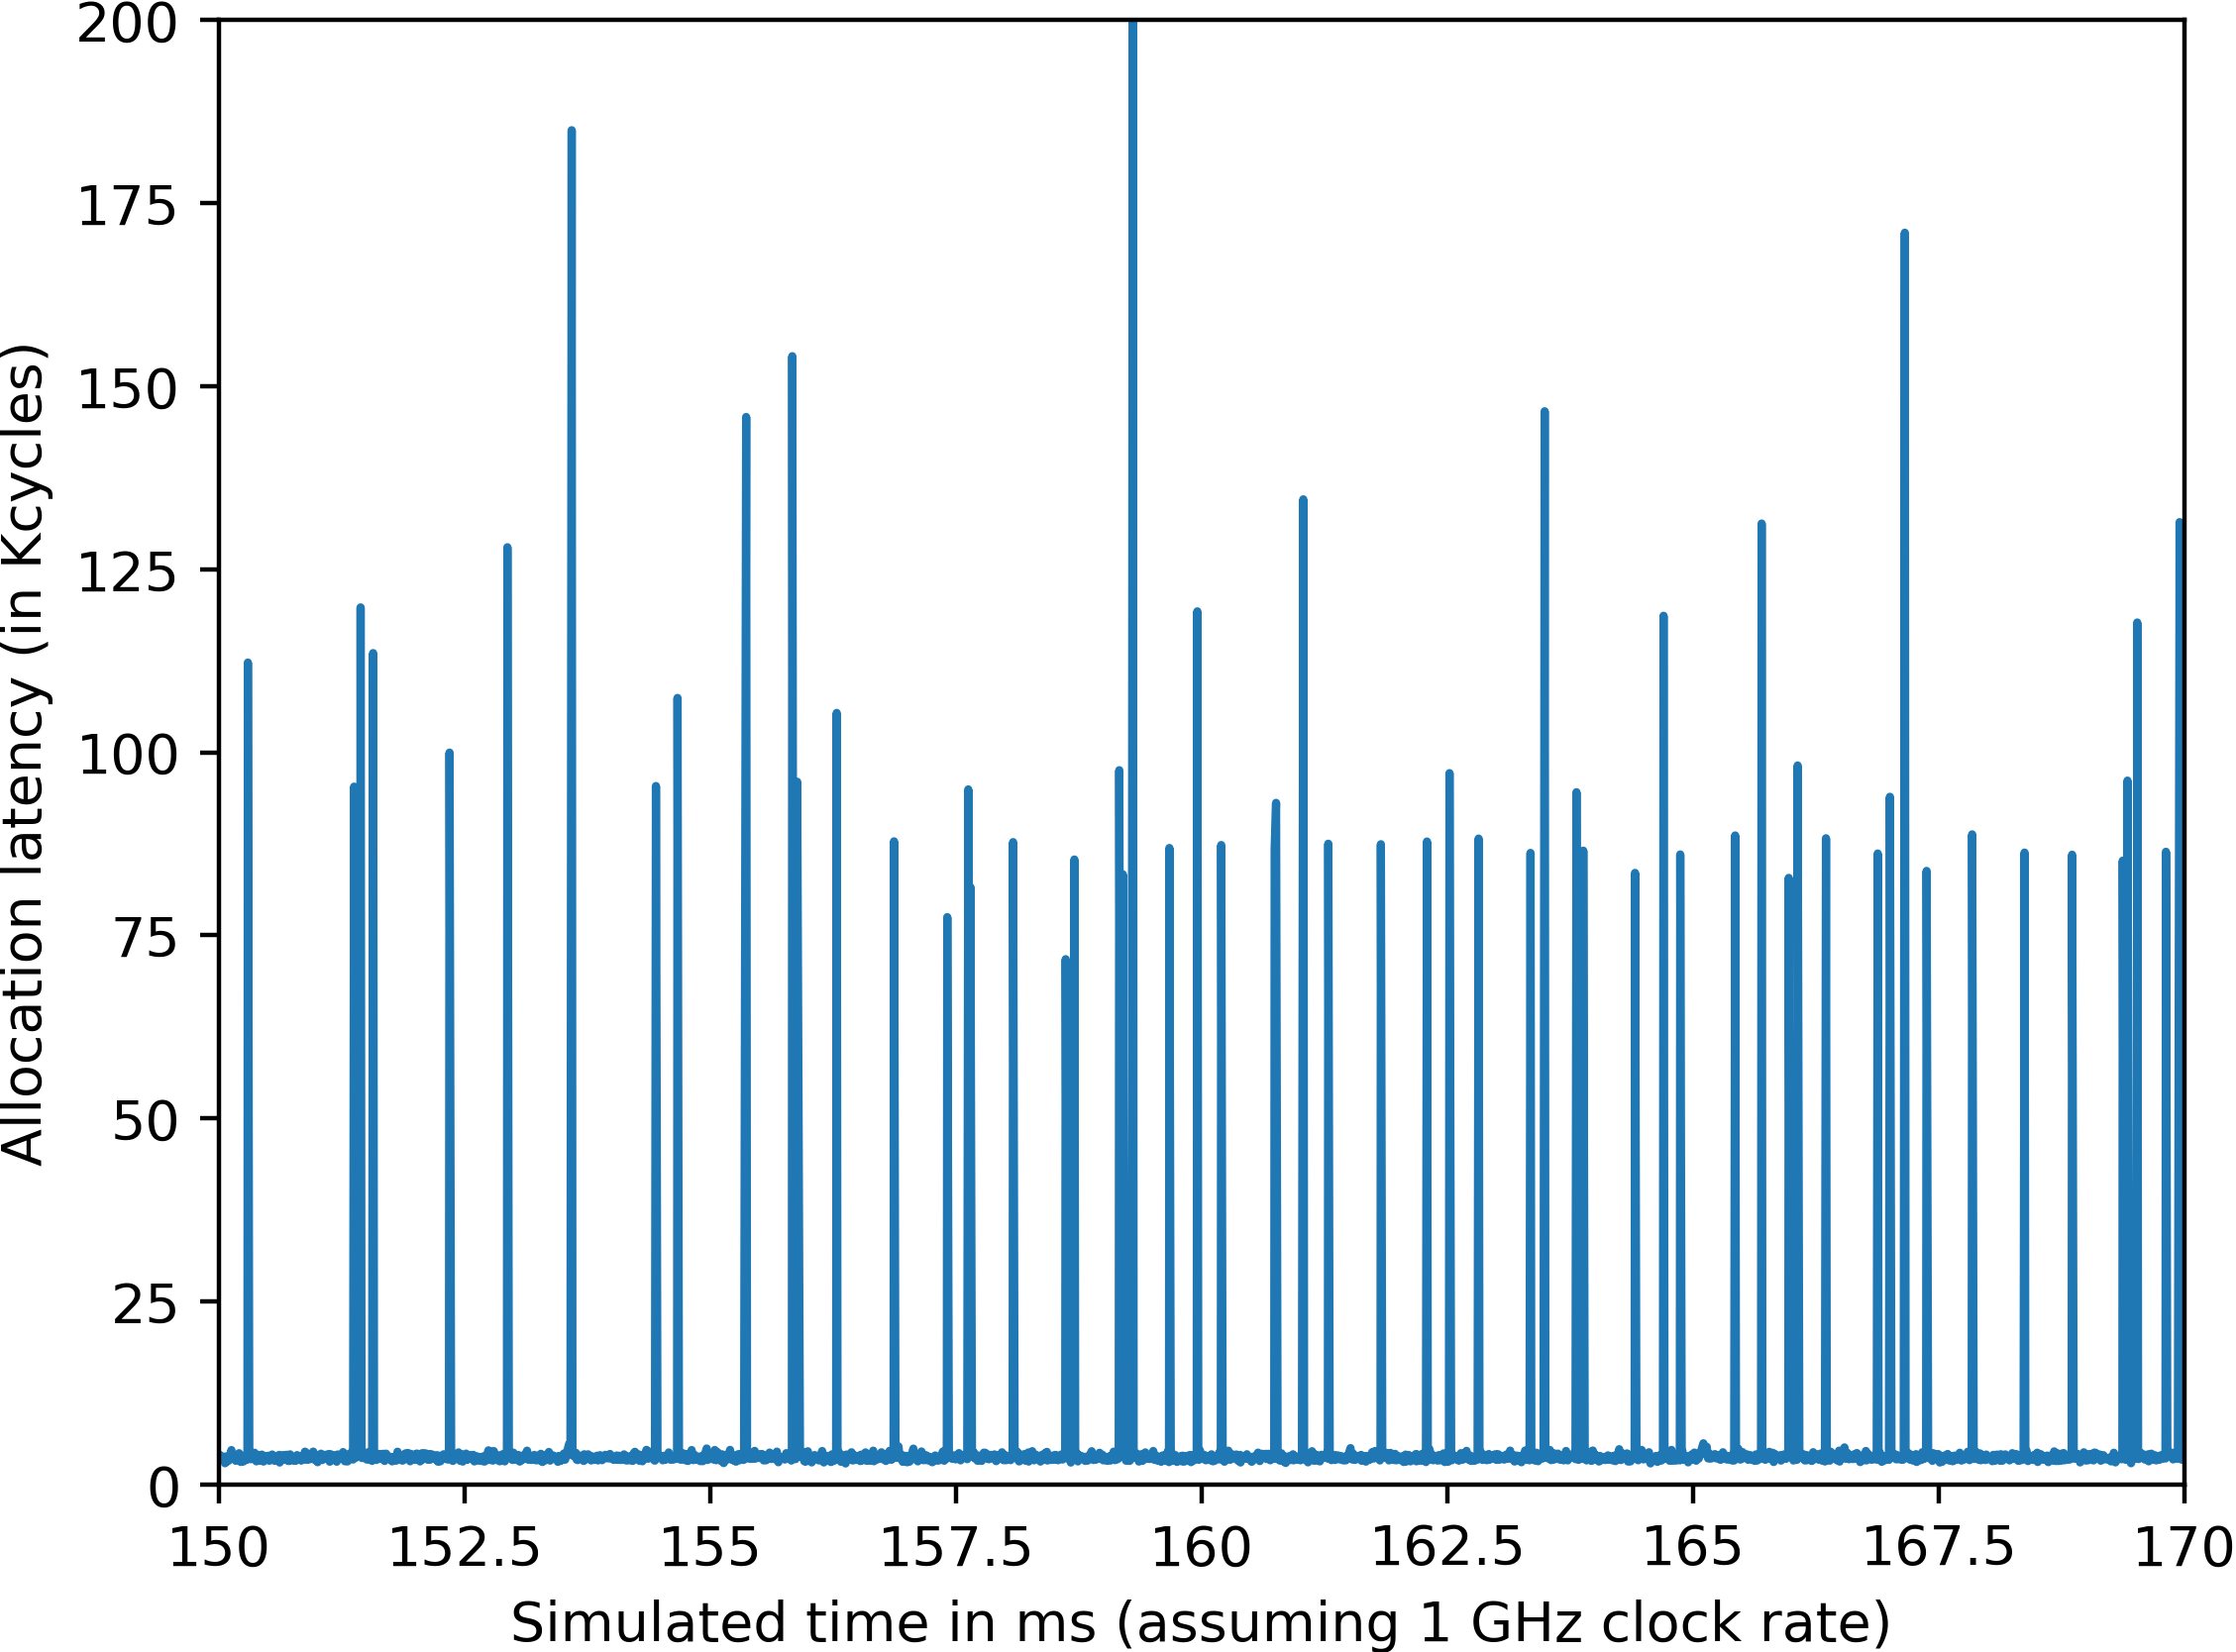
\includegraphics[width=\textwidth]{results/java-alloc-detailed.png}
		\caption{Trace of the same 20ms on our platform}
	\end{subfigure}
	\caption{Contrasting an approach that aggregates time spent in allocation at a 1 KHz-granularity with recording every allocation in hardware without introducing observer effects to the application (numbers are from the \texttt{pmd} DaCapo benchmark).}
	\label{fig:java_alloc}
\end{figure*}

Managed languages such as Java, C\# or Python are widely used and a large
amount of research focuses on improving the language runtime systems that
underpin these languages. Previous work suggests that managed-language runtimes
can substantially benefit from hardware support and hardware-software
co-design~\cite{Click:2005:PGA:1064979.1064988,Wright:2005:OMA:1698178,Ungar:1984:ASS:800015.808182,Joao:2009:FRH:1555754.1555806}.


\begin{figure}[t]
		\centering
		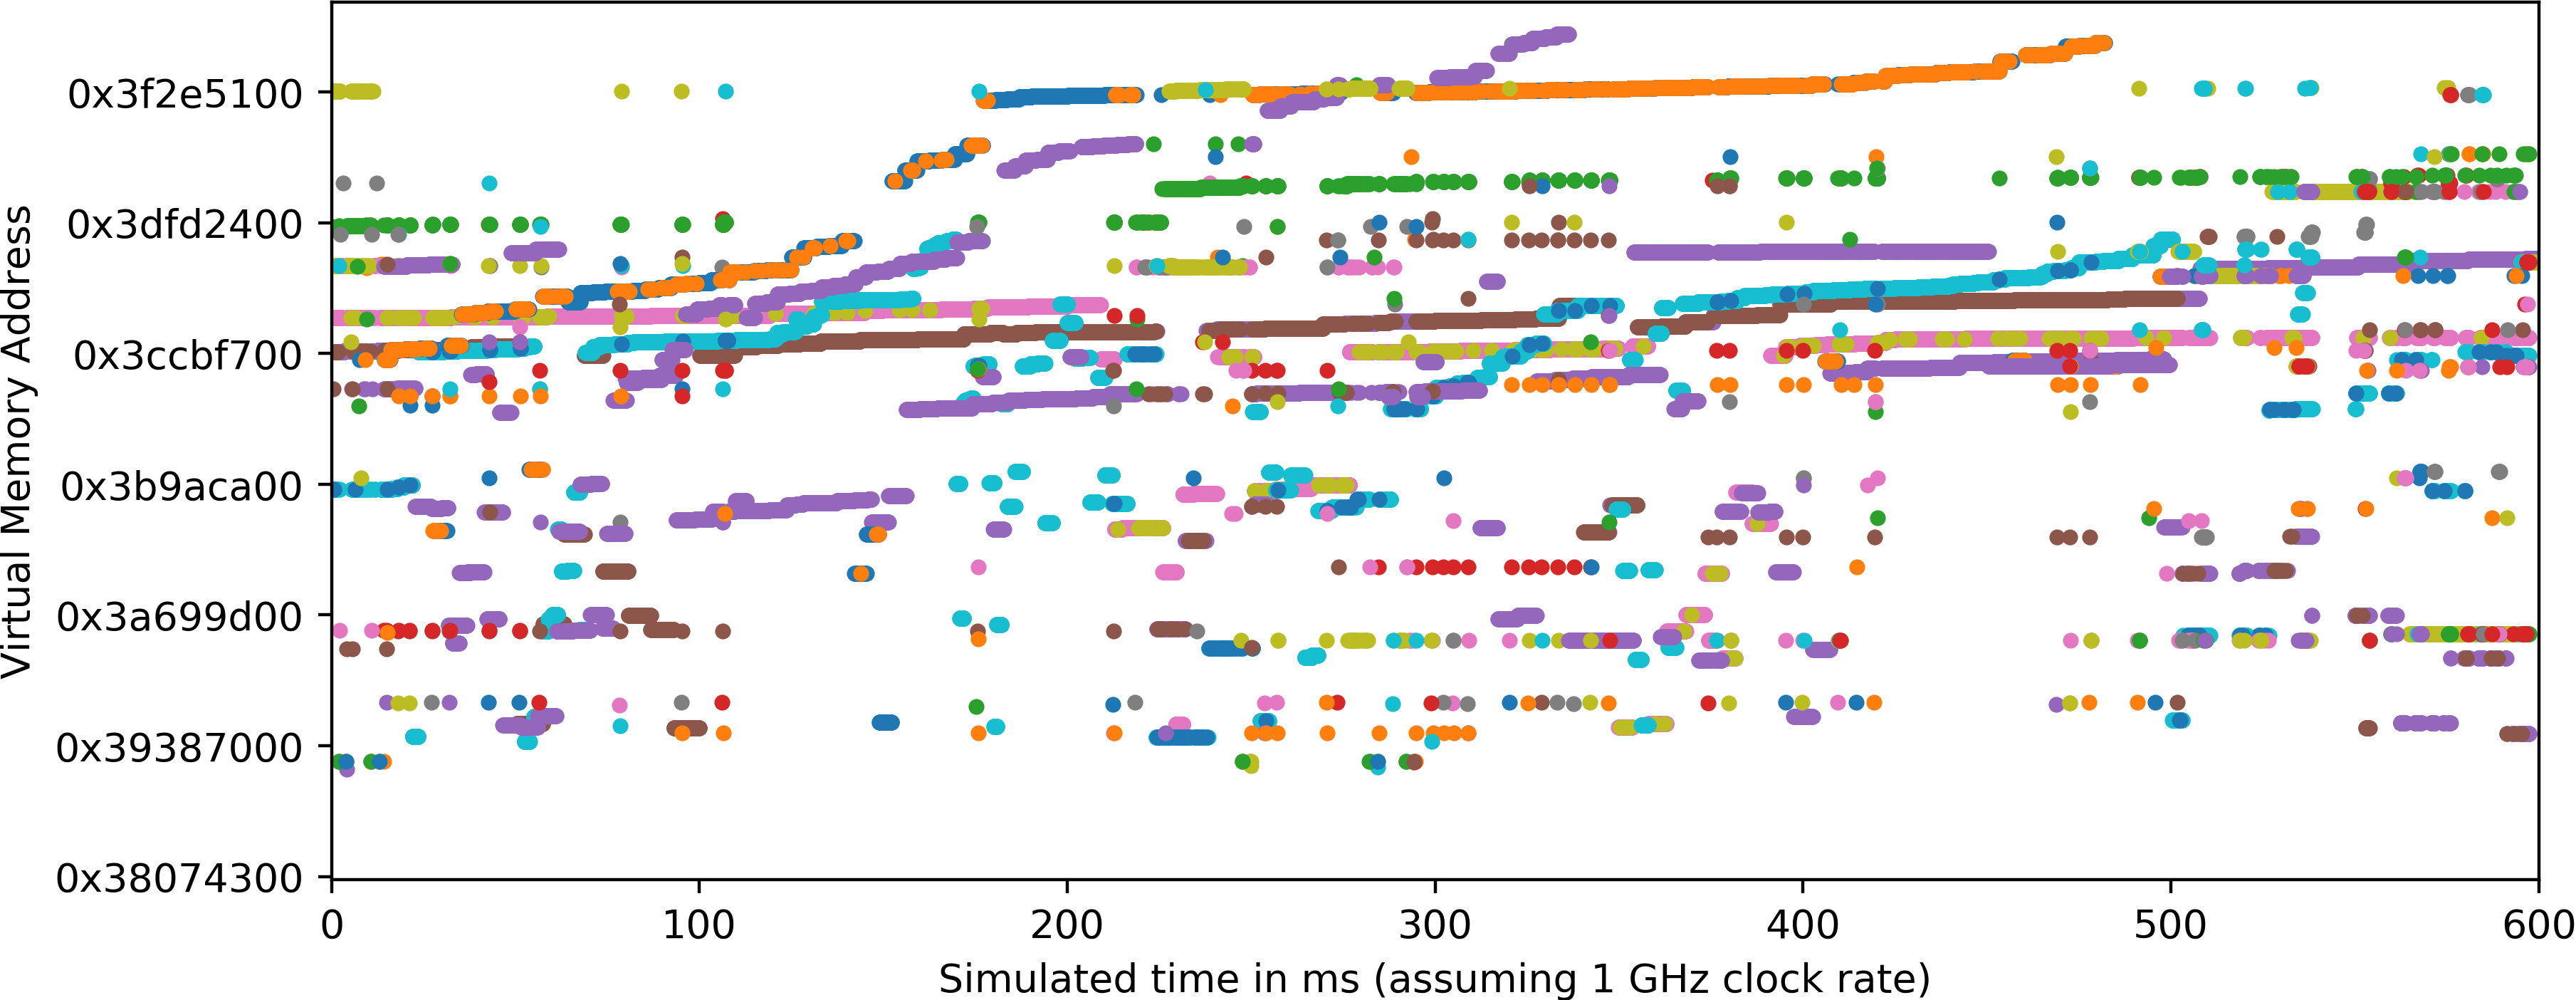
\includegraphics[width=\columnwidth]{results/heatmap.png}
		\caption{Addresses returned by the JikesRVM free-list allocator. Colors indicate the allocation size class.}
		\label{fig:java_alloc_heatmap}
\end{figure}

However, evaluating this work without building out the full system is
challenging, as the interactions between hardware and software are often very
fine-grained and can therefore only be captured in high-fidelity simulation.
For example, concurrent garbage collectors incur most of their overheads from
code sequences that individually only account for 10 or less cycles, but occur
on every reference access~\cite{Click:2005:PGA:1064979.1064988}. In a different
line of work, Yang et al. demonstrated that sampling Java applications at 100
KHz or less misses many important performance characteristics
\cite{Yang:2015:CPM:2749469.2750401}.


\begin{figure}[t]
		\centering
		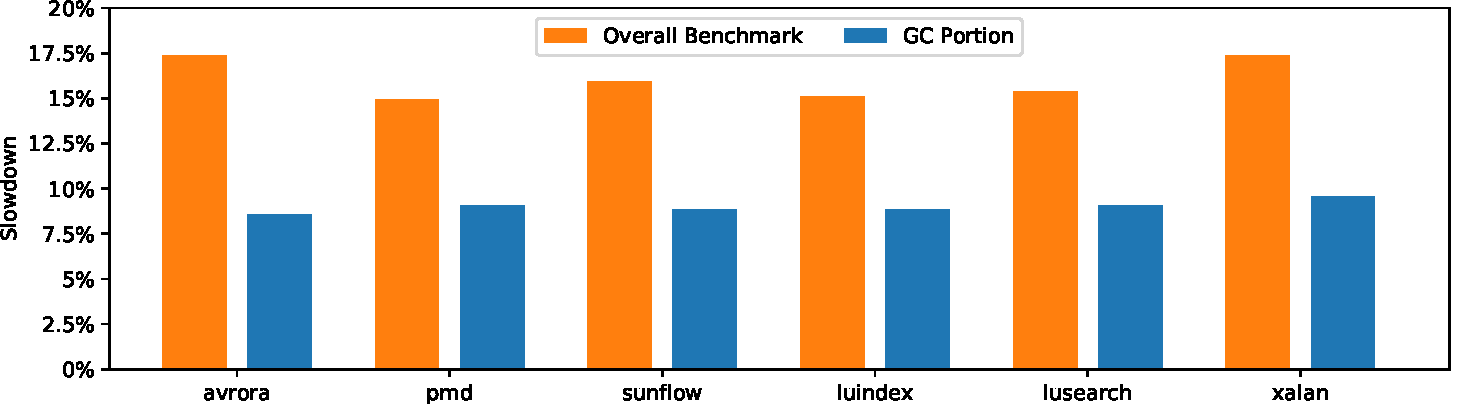
\includegraphics[width=\columnwidth]{results/dacapo-varymodel.pdf}
		\caption{Slowdown of increasing DRAM latency by a factor of 2$\times$. Breaking out the data into GC and non-GC portion shows us that the GC is less sensitive to long memory latencies than the rest of the execution.}
		\label{fig:dacapo_latency2x}
\end{figure}

While high-fidelity software simulators would solve these problems, managed
workloads run across a large number of threads and require full-system support,
which makes them unsuitable for existing simulators. Java workloads in
particular also have very large memory footprints. As a result, extensive
design space explorations that involve managed languages are rare, and recent
work has instead focused on better measuring existing hardware~\cite{Cao:2012:YYP:2337159.2337185,Yang:2015:CPM:2749469.2750401}.

One example of these types of challenges are exemplified in a paper by Hertz
and Berger~\cite{Hertz:2005:QPG:1094811.1094836}. In order to investigate
trade-offs between manual and automatic memory management, the authors had to
instrument an existing system to extract allocated memory addresses, and -- in
a second pass -- inject addresses produced by an oracle. The authors found that
this was difficult to achieve in software, as the software instrumentation led
to a 2-33\% perturbation in execution time, which was larger than the effect
they were trying to measure. They therefore decided to use a software simulator
(Dynamic SimpleScalar) for these experiments. While appropriate in this
setting, the shortcoming of this approach is simulation speed and the
reliability of the resulting numbers.

FPGA simulations, automatically generated from the RTL designs~\cite{strober},
in conjunction with the realistic memory models introduced in this paper,
provide an opportunity to fundamentally address this problem by running on real
hardware that can be modified and enables design space exploration of the
memory and I/O system. The memory system is particularly important, as many
managed-runtime problems are closely interlinked with it (e.g., memory
allocation or GC).

To enable this kind of research, we brought up a full Java Virtual Machine
(JVM) on our platform. We picked the Jikes Research
VM~\cite{alpern_jikes_2005}, which is the de facto standard in managed-language
research. We ported JikesRVM and its non-optimizing \emph{Baseline} JIT
compiler to RISC-V. To our knowledge, this is the first full-system platform
for hardware-software research on Java applications, allowing modification of
the software stack, the hardware and the memory system model. Larger FPGAs with
several GBs of DRAM (which only became available recently) were essential in
enabling this. In the following sections, we will describe the types of
experiments that become possible with our platform.


\begin{figure*}
	\centering
	\begin{subfigure}[t]{0.23\textwidth}
		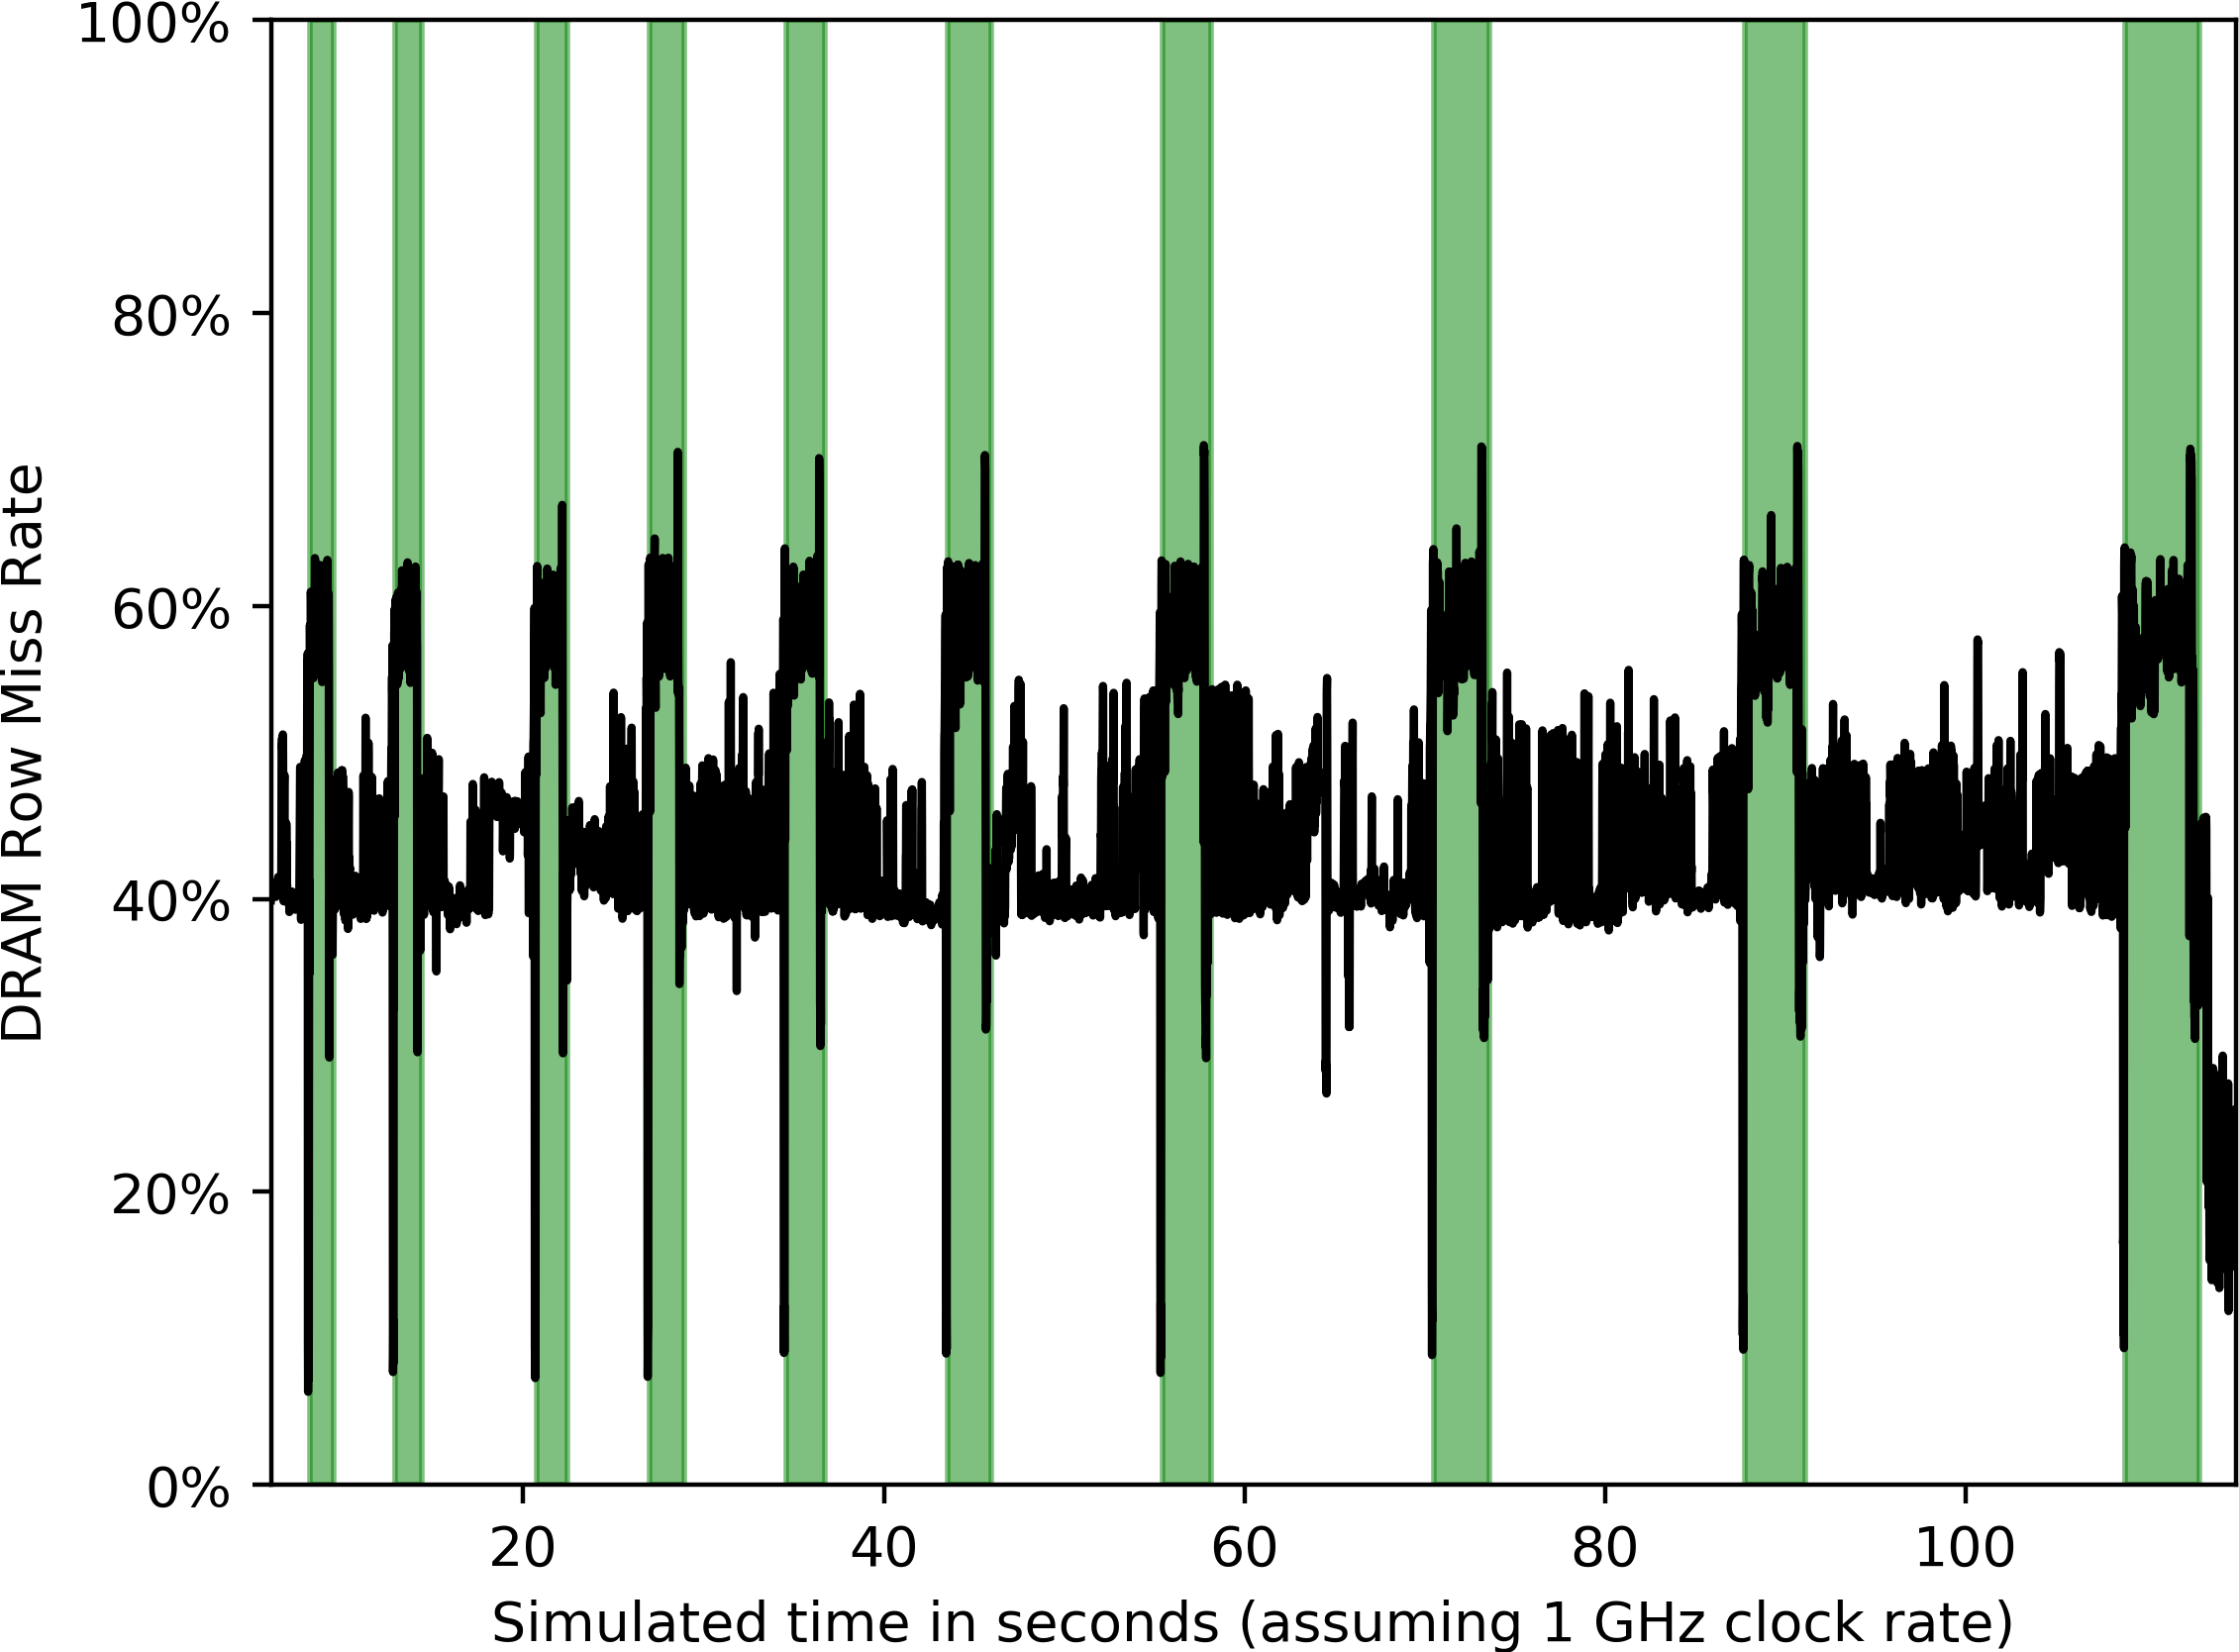
\includegraphics[width=\textwidth]{results/rowmisses_pmd.png}
		\caption{pmd}
	\end{subfigure}
	\begin{subfigure}[t]{0.23\textwidth}
		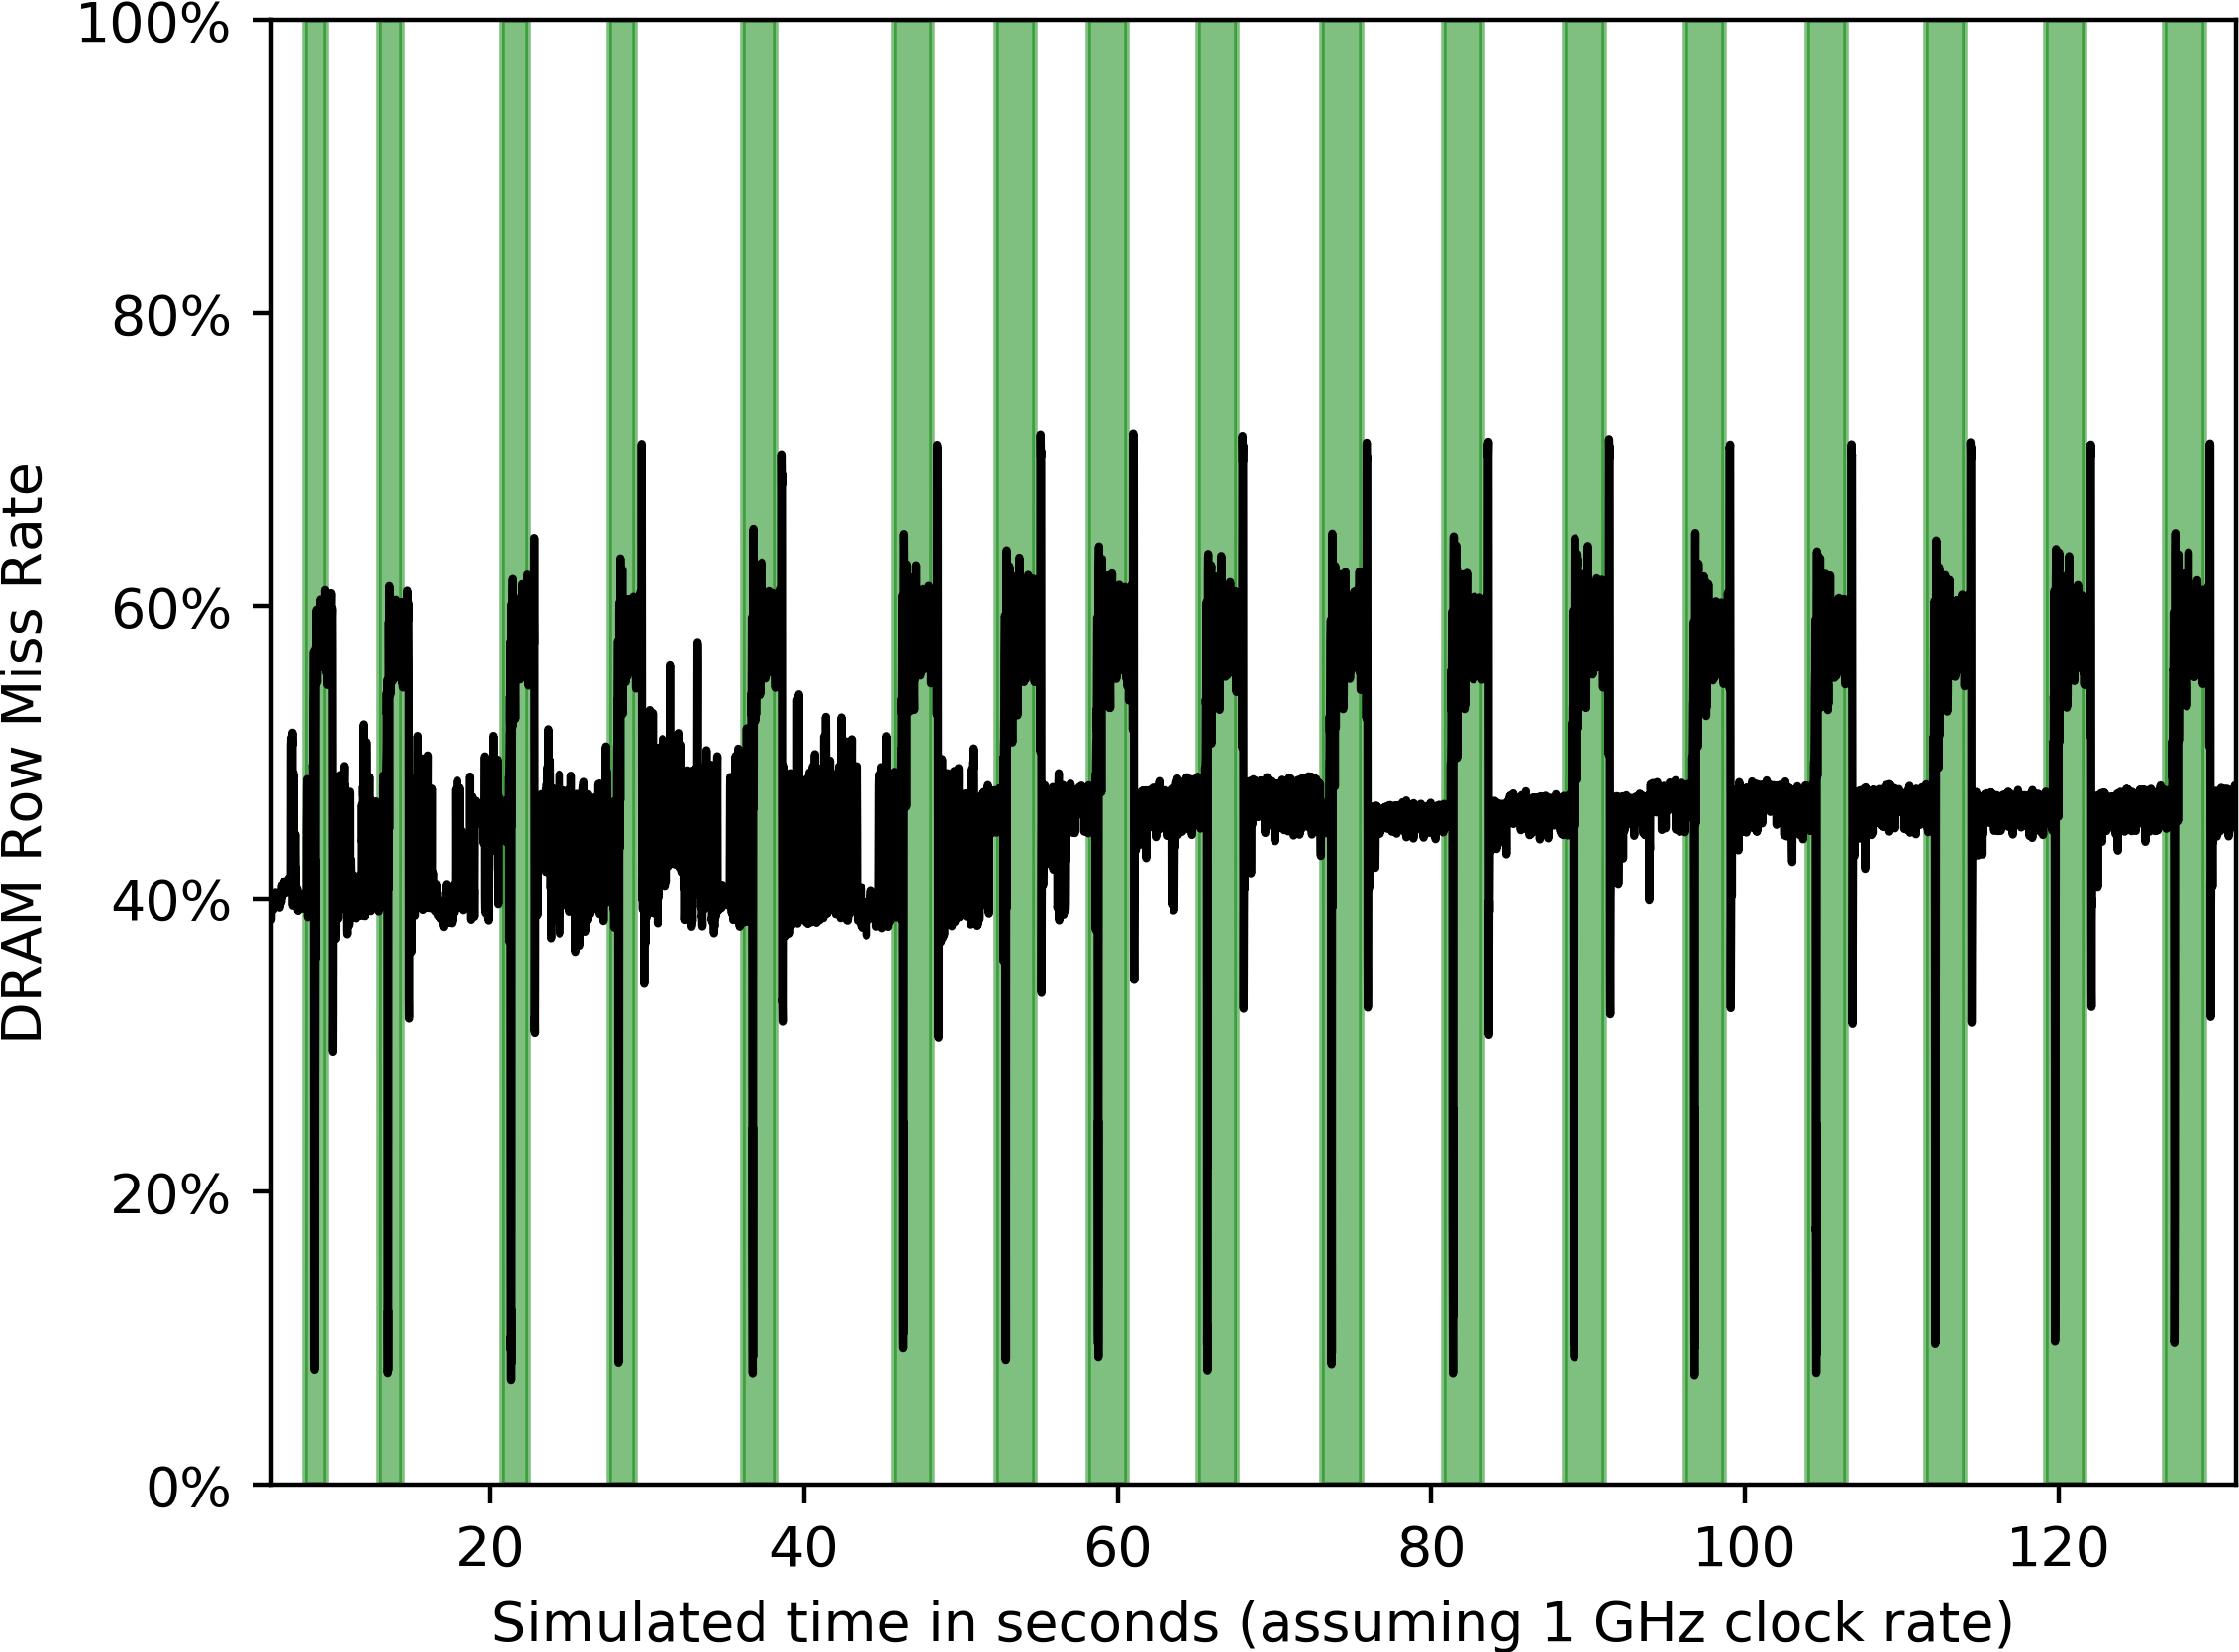
\includegraphics[width=\textwidth]{results/rowmisses_lusearch.png}
		\caption{lusearch}
	\end{subfigure}
	\begin{subfigure}[t]{0.23\textwidth}
		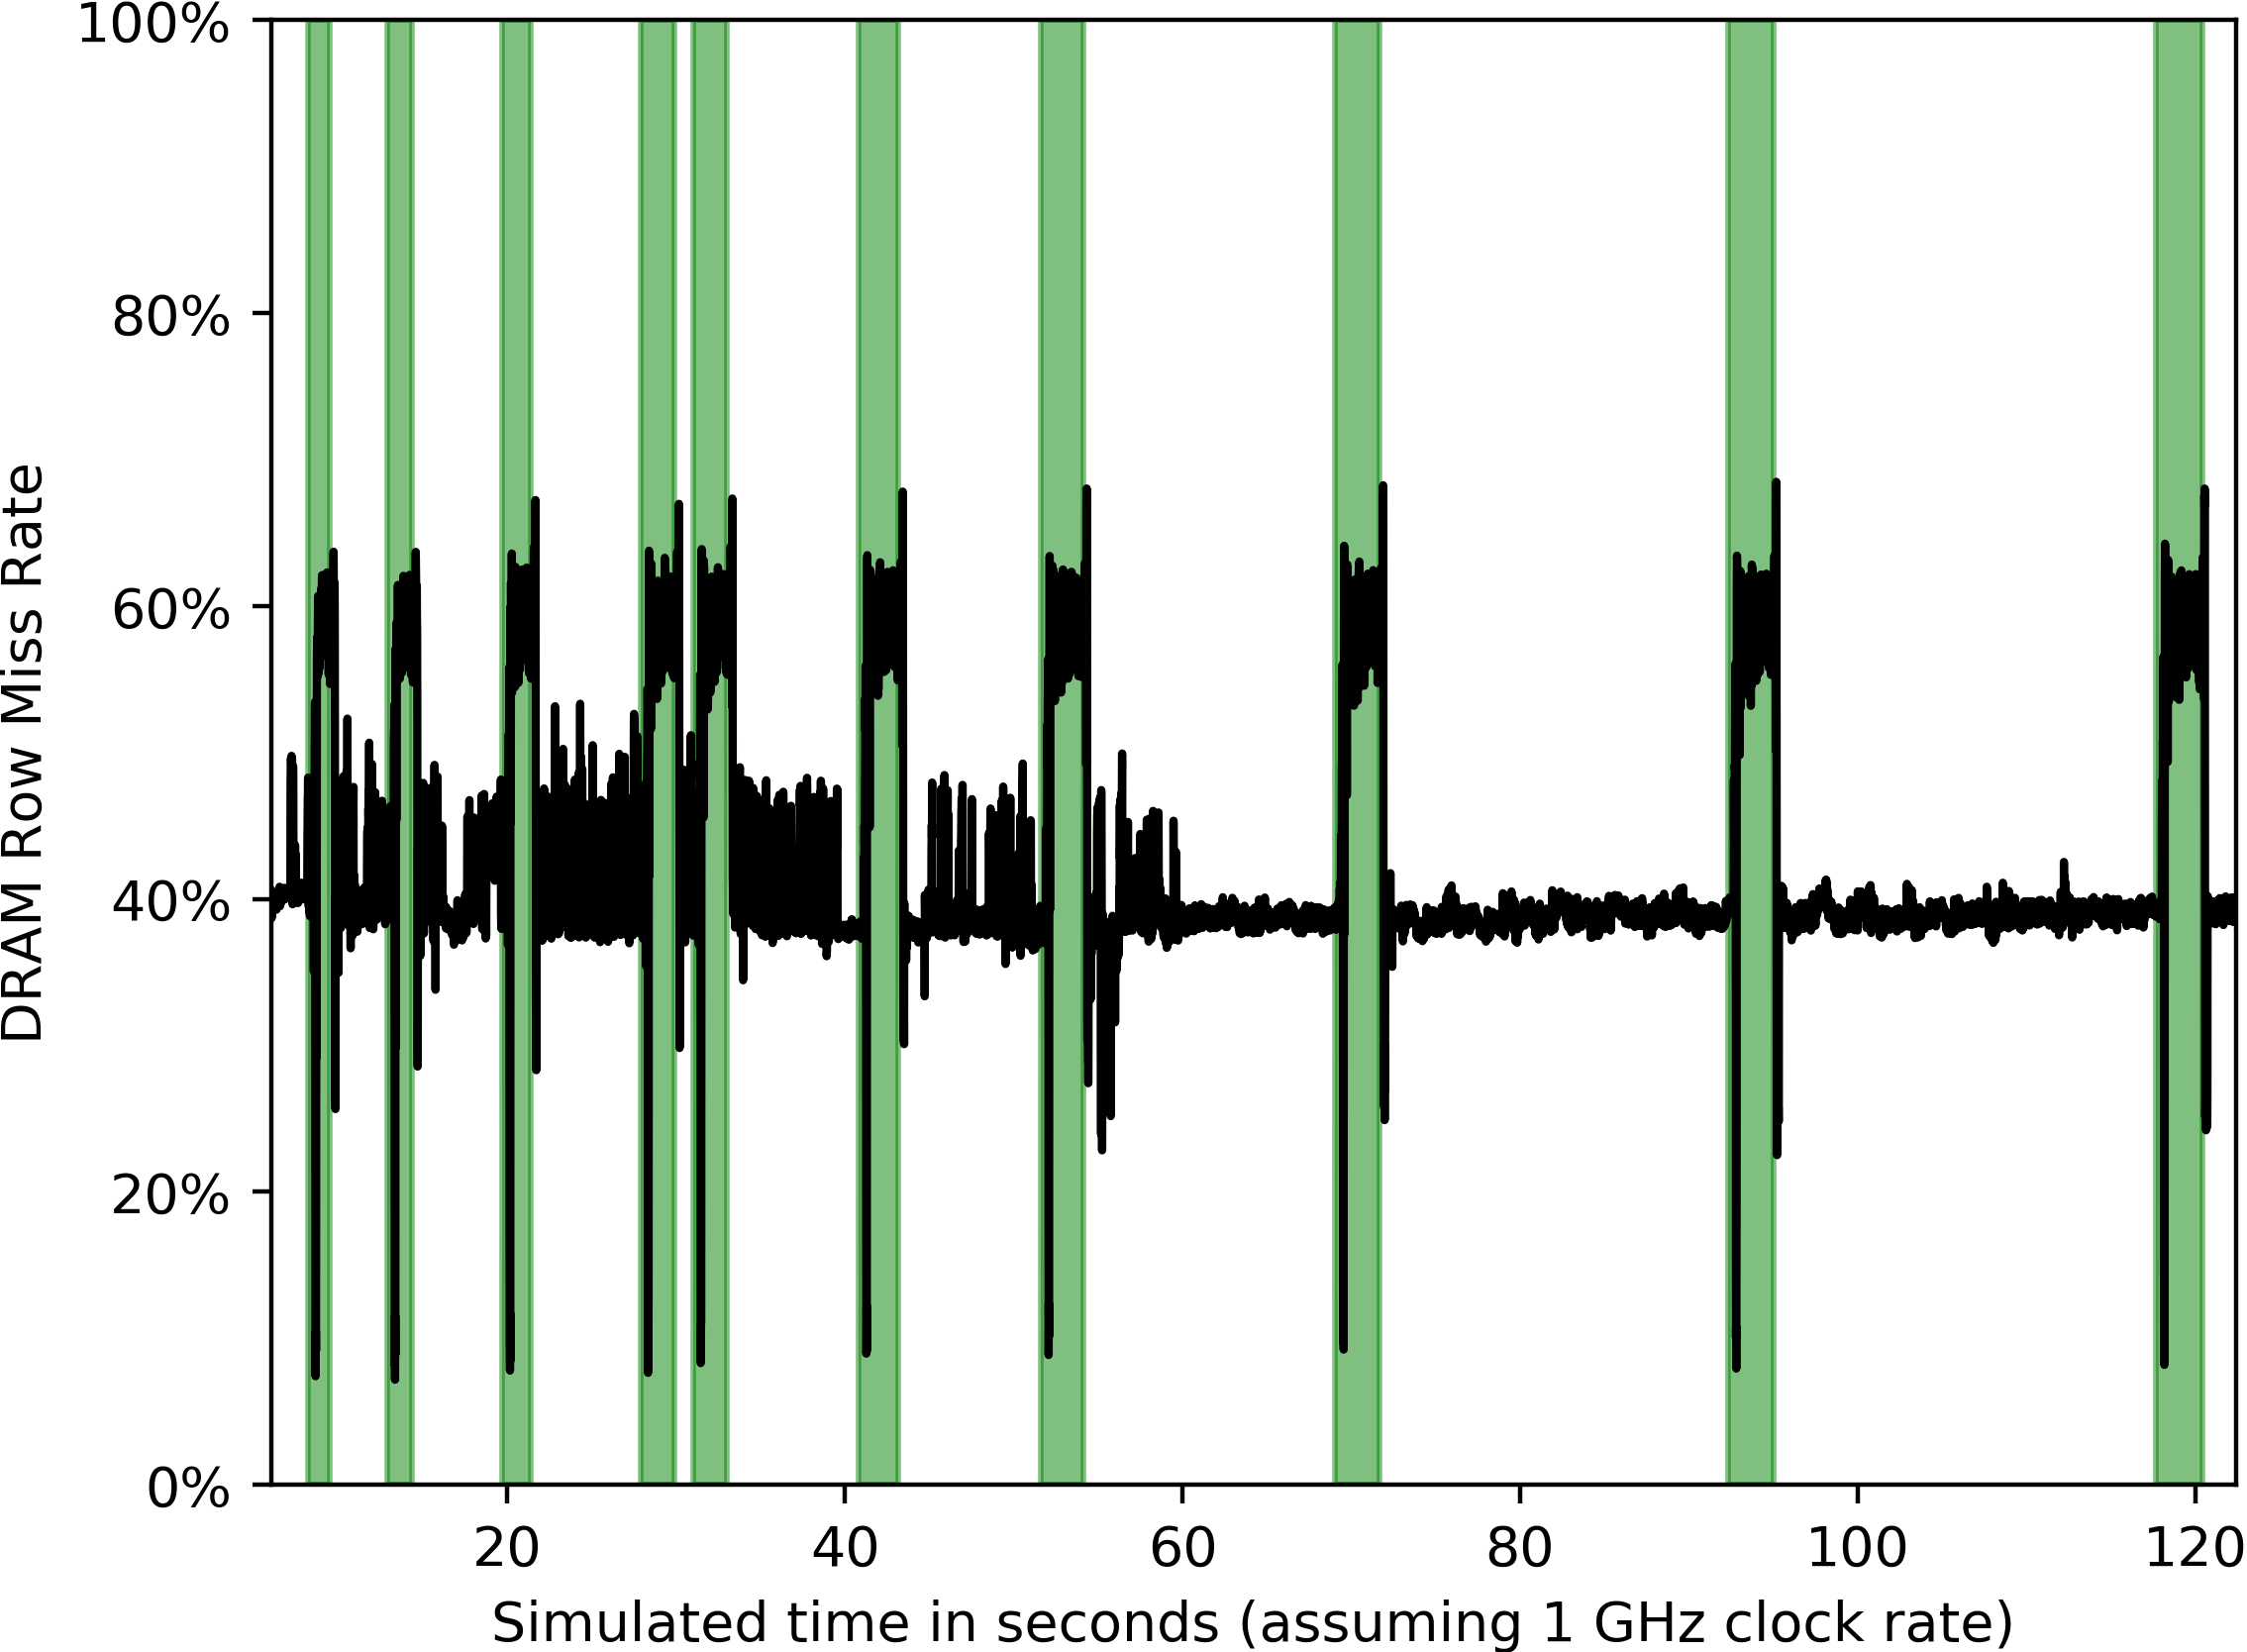
\includegraphics[width=\textwidth]{results/rowmisses_sunflow.png}
		\caption{sunflow}
	\end{subfigure}
	\begin{subfigure}[t]{0.23\textwidth}
		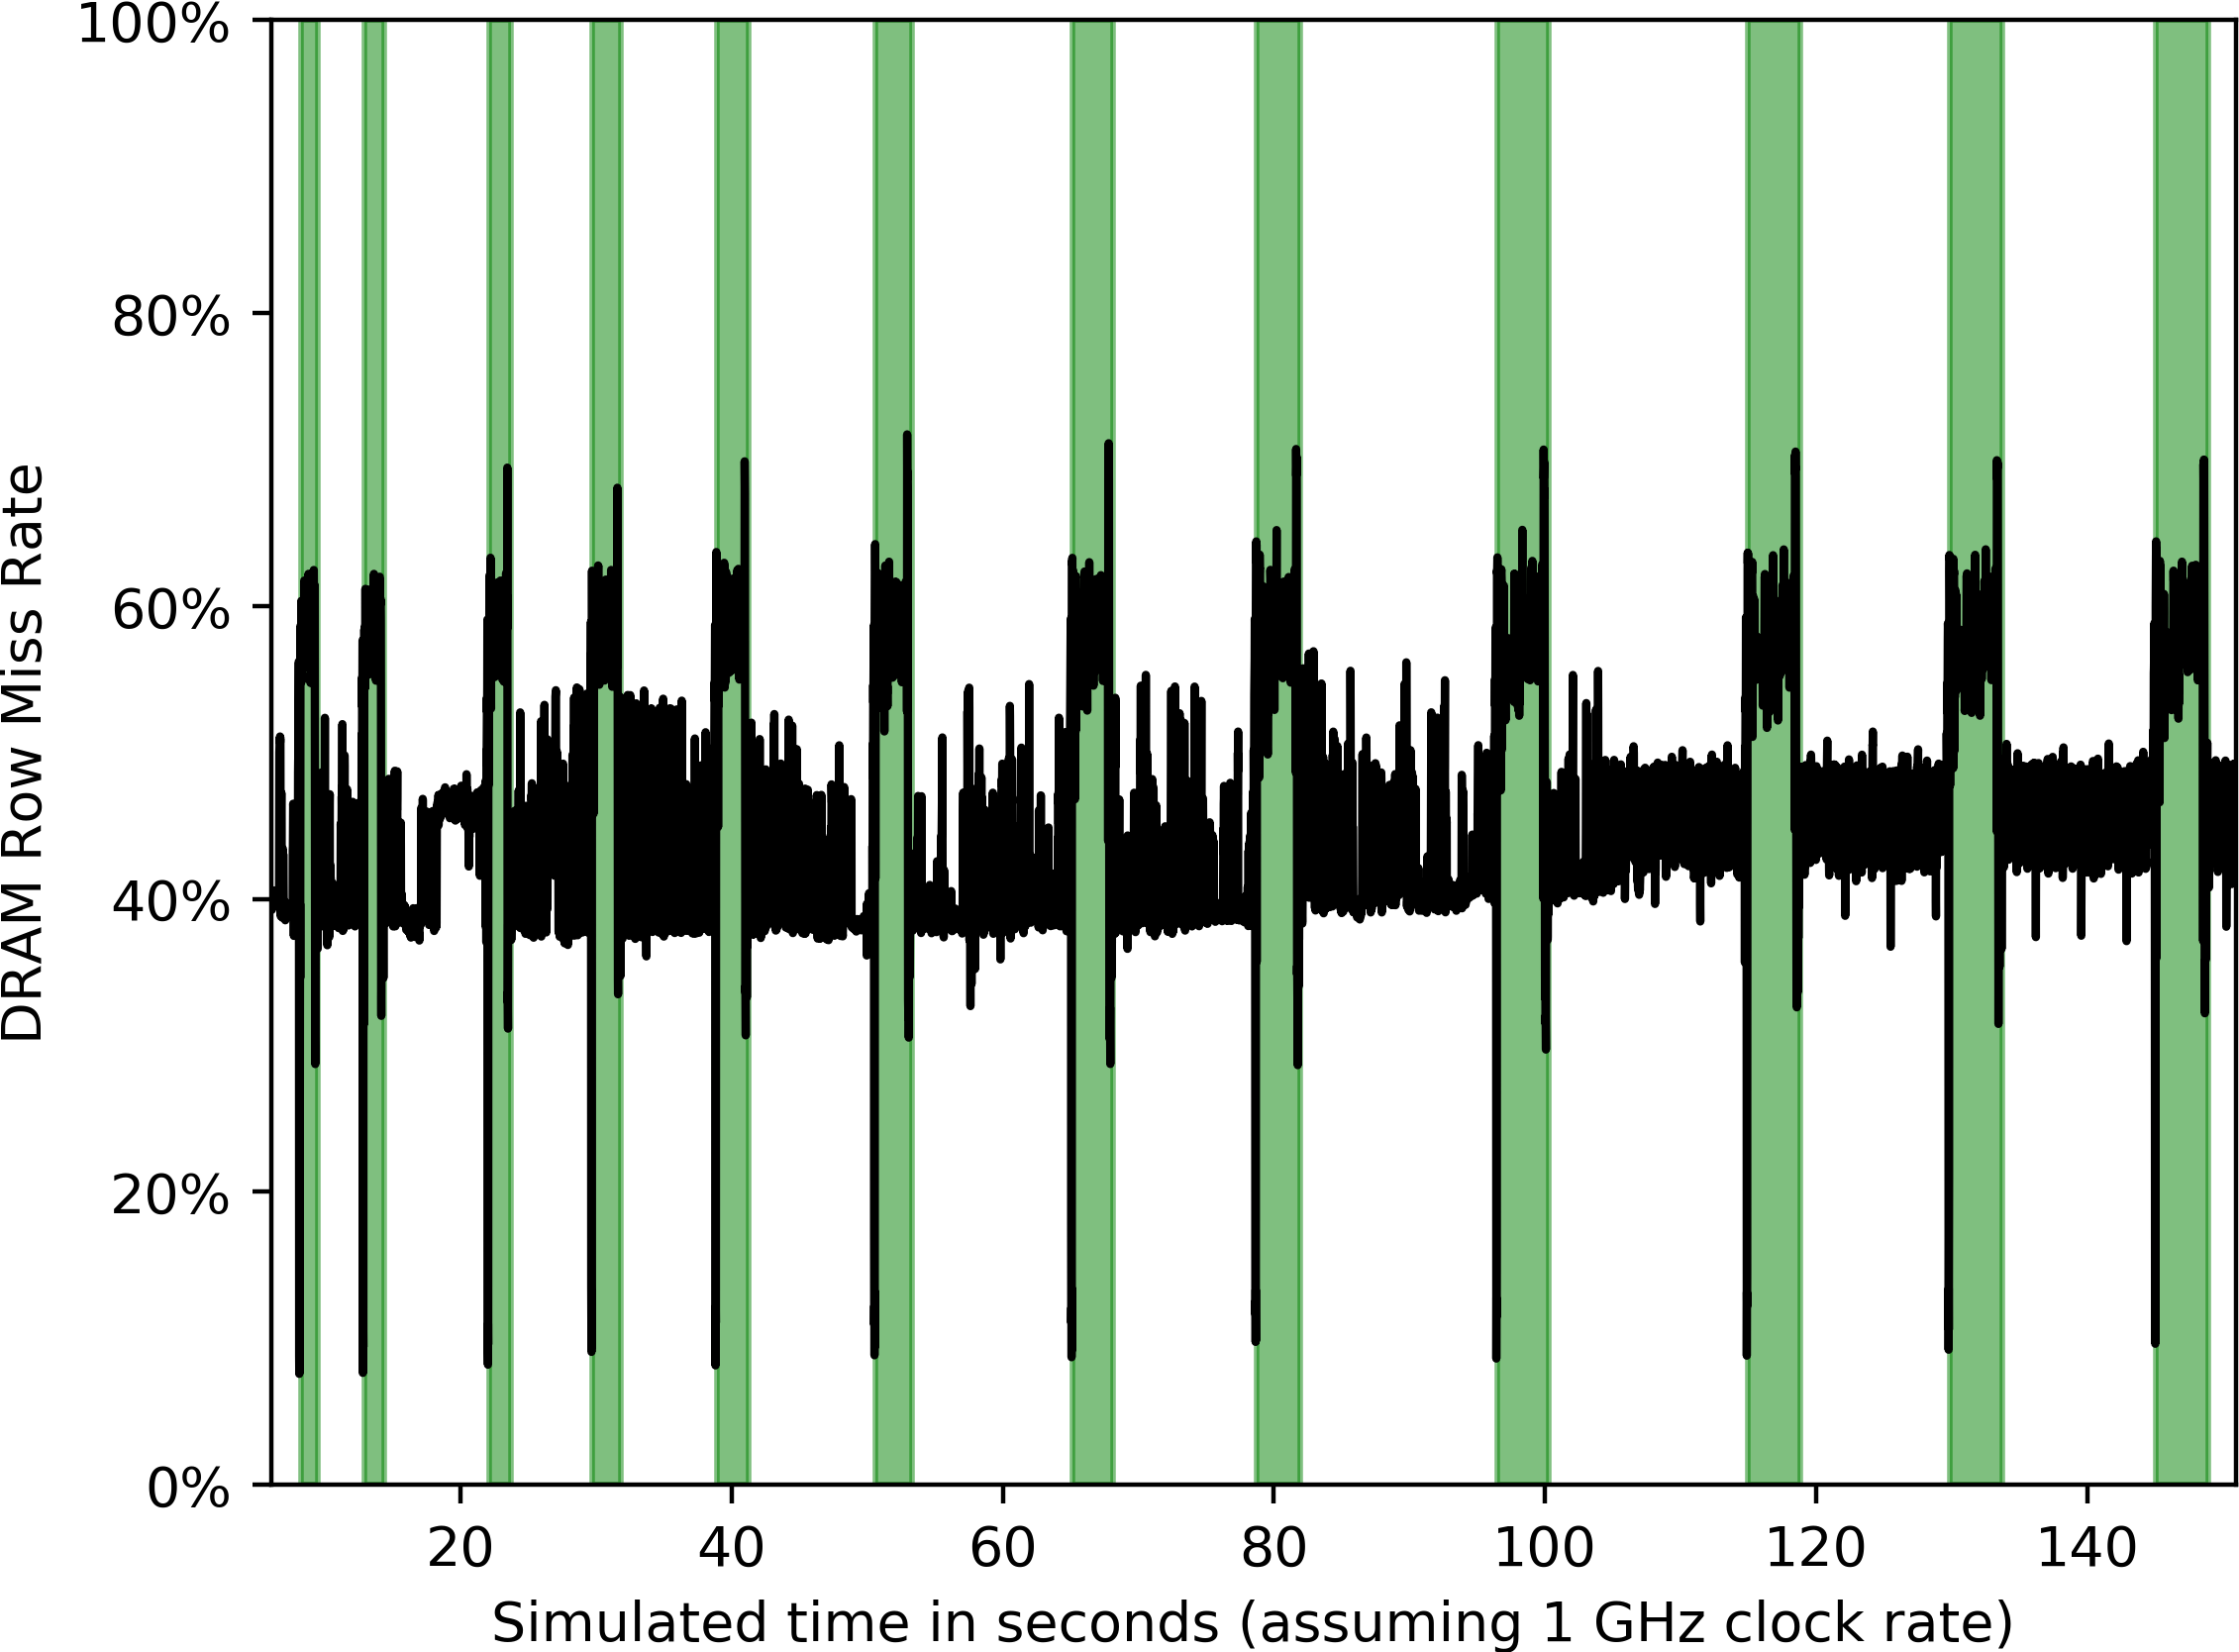
\includegraphics[width=\textwidth]{results/rowmisses_xalan.png}
		\caption{xalan}
	\end{subfigure}
    \caption{Running the DaCapo Java benchmarks and plotting the percentage of
    memory accesses that incur a DRAM row miss with the FCFS open-row DRAM
    model. While their behavior differs substantially, Garbage Collection
    phases are immediately visible (shown in green): due to their very low
    locality, they have a much lower hit rate than the rest of the application,
    and at the beginning of each GC phase, there is a brief period with a very
    high hit rate -- namely, the sequential scanning of the application's
    stacks to identify all references contained in them (i.e., roots).}
	\label{fig:java_rowmisses}
\end{figure*}

\section{High-Fidelity Application Traces}

To demonstrate the capabilities of our platform, we ran an experiment where we
annotated all memory allocation operations in JikesRVM to record a trace of
both the sizes that are being allocated and the virtual addresses that are
being returned. We buffer this (long) trace in block RAMs that we added to the
target RTL design, and read it out through automatically-inserted scan
chains~\cite{strober}.

By using this approach, we can record a trace of every memory allocation
without perturbing the execution of the program\footnote{The same mechanism
could be used to inject precomputed data, although this is currently not
implemented.}. To collect this data on a conventional system, we would need to
use either software-based sampling or code instrumentation. The latter
inherently adds observer effects and is therefore unsuitable to measure
fine-grained effects. While it was recently shown that sampling can collect
hardware-performance counters at a 1,200 cycle resolution on modern x86
cores~\cite{Yang:2015:CPM:2749469.2750401}, these approaches cannot collect
application-level details, such as allocated addresses or allocation sizes
(i.e., state contained the register file).

The fidelity of this data enables us to see effects that would be hidden by
less-detailed measurements. Figure~\ref{fig:java_alloc} shows a slice of the
$\emph{pmd}$ benchmark with the time spent in allocation aggregated over
1M-cycle intervals (which corresponds to a sampling frequency of 1 KHz). While
this enables us to understand the macro-behavior of the application
(Figure~\ref{fig:java_alloc}a), the data is meaningless when trying to
understand the behavior of individual memory allocations
(Figure~\ref{fig:java_alloc}b). In contrast, the detailed data collected in our
system (Figure~\ref{fig:java_alloc}c) shows us a much more interesting
behavior: most allocations take a small amount of time ($\approx 4,000$
cycles), while occasional allocations take $10-100\times$ longer. This is
anticipated: the memory allocator is a segregated free list allocator and the
allocator's fast path consumes a per-size-class free list. As soon as the free
list is used up, the allocator has to fetch a new block from the global block
free list, which involves zeroing the block's memory. Dividing the allocation
trace by size class, we can measure the number of allocations to the same size
class between slow path invocations, which allows us to deduce the amount of
memory fragmentation, which would not have been visible from lower-fidelity
measurements.


Other information we can learn from this trace are allocation rates, the
distribution of allocated memory sizes and the pattern of allocated addresses:
in particular, we are often interested in the locality of subsequent memory
addresses assigned by the allocator, as this has been shown to be crucial for
performance~\cite{Blackburn:2004:OWH:998675.999420}.
Figure~\ref{fig:java_alloc_heatmap} shows the addresses generated by the
allocation, colored according to the size of the allocated object. What we can
see is that while allocation of the same object sizes is usually contiguous
(until the end of the free list is reached and a new block is acquired), the
overall temporal locality is low, confirming the conventional wisdom that
free-list allocators produce poor locality~\cite{Blackburn:2004:OWH:998675.999420}.

\section{Varying the DRAM Timing Model}

Managed runtime systems are often sensitive to the underlying
hardware~\cite{Cao:2012:YYP:2337159.2337185}. Using our platform, it is
possible to vary the details of the underlying memory system, and explore their
impact on the application.

We ran an experiment where we measured the impact of doubling the memory
latency for the FCFS MAS timing-model with open page policy from
Table~\ref{tbl:fcfs-programmable-registers} (Figure~\ref{fig:dacapo_latency2x}). This allowed us
to understand how sensitive different phases of the language runtime system are
to memory latencies.

These experiments taught us that the GC phase is substantially less affected by
high memory latencies than the rest of the application. This was surprising to
us, as the GC consists mainly of a pointer chase and should therefore be
strongly affected by the latency. However, upon closer investigation, we
discovered that each GC step involved not only following an object reference
but also parsing the object, identifying its outbound references and enqueuing
these references to a queue that is resident in the cache. With a trace-based
JIT-compiler, these operations would be inlined, but with a non-optimizing JIT,
they turn into a large number of function calls with high cache hit rates.

This confirms a similar result regarding non-optimized managed code by Cao et
al.~\cite{Cao:2012:YYP:2337159.2337185}. We found the fact that our platform
allowed us to identify this somewhat counter-intuitive effect encouraging.

\section{Recording Memory System Metrics}

Finally, by running with one of our detailed memory models, we can gain deeper
insights into the application behavior than on a traditional system. To
demonstrate this, we ran several DaCapo benchmarks with the FCFS timing-model
and an open-row policy. We recorded the fraction of DRAM accesses that incurred
a row miss (Figure~\ref{fig:java_rowmisses}).

This exhibited an interesting effect: although each application has a very
different behavior, we can see that all benchmarks periodically exhibit a very
distinctive pattern of row miss rates: a large spike of brief, low row miss
rates, followed by a period of very high miss rates. By correlating this
behavior to the application output, we identified that these were the garbage
collection phases in the application.

Specifically, at the beginning of each GC phase, the JVM has to sequentially
scan the application's stacks and global variables, which are long, sequential
accesses that substantially benefit from an open-row policy. This is followed
by a phase of pointer-chasing -- while we saw in the previous section that many
memory accesses during this phase hit in the cache, those that do go through to
main memory rarely hit an open row, because of the very limited locality during
the tracing phase.

By using our memory model and collecting these metrics, we are able to gain
deeper insight into these kinds of effects. This could be a first step towards
modifying the memory system in order to tune it better for managed-language
workloads (e.g., to improve
energy-efficiency~\cite{Cao:2012:YYP:2337159.2337185}). By allowing us to
modify the memory system model, our platform enables this kind of research.
